%%%%%%%%%%%%%%%%%%%%%%%%%%%%%%%%%%%%%%%%%
% Beamer Presentation
% LaTeX Template
% Version 1.0 (10/11/12)
%
% This template has been downloaded from:
% http://www.LaTeXTemplates.com
%
% License:
% CC BY-NC-SA 3.0 (http://creativecommons.org/licenses/by-nc-sa/3.0/)
%
%%%%%%%%%%%%%%%%%%%%%%%%%%%%%%%%%%%%%%%%%

%----------------------------------------------------------------------------------------
%   PACKAGES AND THEMES
%----------------------------------------------------------------------------------------

\documentclass{beamer}

\mode<presentation> {

% The Beamer class comes with a number of default slide themes
% which change the colors and layouts of slides. Below this is a list
% of all the themes, uncomment each in turn to see what they look like.

% \usetheme{default}
% \usetheme{AnnArbor}
% \usetheme{Antibes}
% \usetheme{Bergen}
% \usetheme{Berkeley}
% \usetheme{Berlin}
% \usetheme{Boadilla}
% \usetheme{CambridgeUS}
% \usetheme{Copenhagen}
% \usetheme{Darmstadt}
% \usetheme{Dresden}
% \usetheme{Frankfurt}
% \usetheme{Goettingen}
% \usetheme{Hannover}
% \usetheme{Ilmenau}
% \usetheme{JuanLesPins}
% \usetheme{Luebeck}

\usetheme{Madrid}

% \usetheme{Malmoe}
% \usetheme{Marburg}
% \usetheme{Montpellier}
% \usetheme{PaloAlto}
% \usetheme{Pittsburgh}
% \usetheme{Rochester}
% \usetheme{Singapore}
% \usetheme{Szeged}
% \usetheme{Warsaw}

% As well as themes, the Beamer class has a number of color themes
% for any slide theme. Uncomment each of these in turn to see how it
% changes the colors of your current slide theme.

% \usecolortheme{albatross}
% \usecolortheme{beaver}
% \usecolortheme{beetle}
% \usecolortheme{crane}

\usecolortheme{dolphin}

% \usecolortheme{dove}
% \usecolortheme{fly}
% \usecolortheme{lily}
% \usecolortheme{orchid}
% \usecolortheme{rose}
% \usecolortheme{seagull}
% \usecolortheme{seahorse}
% \usecolortheme{whale}
% \usecolortheme{wolverine}

%\setbeamertemplate{footline} % To remove the footer line in all slides uncomment this line
%\setbeamertemplate{footline}[page number] % To replace the footer line in all slides with a simple slide count uncomment this line

%\setbeamertemplate{navigation symbols}{} % To remove the navigation symbols from the bottom of all slides uncomment this line
}

\usepackage{graphicx} % Allows including images
\usepackage{booktabs} % Allows the use of \toprule, \midrule and \bottomrule in tables
\usepackage[draft]{todonotes}

\usepackage[utf8]{inputenc}
\usepackage{algorithm}
\usepackage[noend]{algpseudocode}
%----------------------------------------------------------------------------------------
%   TITLE PAGE
%----------------------------------------------------------------------------------------

\title[TP3]{Métodos Numéricos \\ TP3} % The short title appears at the bottom of every slide, the full title is only on the title page

\author{Seijo, De Bortoli, Penas, Grings} % Your name
\institute[DC] % Your institution as it will appear on the bottom of every slide, may be shorthand to save space
{
% FCEN - UBA \\ % Your institution for the title page
% \medskip
% \textit{jon.seijo@gmail.com} % Your email address
}

% \date{\today} % Date, can be changed to a custom date
\date{Noviembre 2017} % Date, can be changed to a custom date

\begin{document}

\begin{frame}
\titlepage % Print the title page as the first slide
\end{frame}

% \begin{frame}
% \frametitle{Overview} % Table of contents slide, comment this block out to remove it
% \tableofcontents % Throughout your presentation, if you choose to use \section{} and \subsection{} commands, these will automatically be printed on this slide as an overview of your presentation
% \end{frame}

%----------------------------------------------------------------------------------------
%   PRESENTATION SLIDES
%----------------------------------------------------------------------------------------

%------------------------------------------------
% \section{Introducción} % Sections can be created in order to organize your presentation into discrete blocks, all sections and subsections are automatically printed in the table of contents as an overview of the talk
%------------------------------------------------


% -----------------------------------

\begin{frame}


% Hicimos scripts en bash para filtrar los datos,
% por ejemplo podiamos filtrar todos los vuelos de tal aerolinea,
%         que salieron del aeropuerto tal, que se cancelo por tal
% Hacer estos scripts de forma generica nos permitio que no nos tengamos que preocupar en pensar como filtrar los datos cada vez, bla


% Usamos python porque era sencillo, ya lo veniamos usando en otros tps. bla bla python esta re bueno because reasons

% Nos aseguramos que la libreria dijera explicitamente que usaba cuadrados minimos
%                           "Ordinary least squares Linear Regression"
% La utilizamos tanto para la aproximacion como por la prediccion, dar credito a la clase de francisco

\frametitle{Sobre los datos}
\begin{itemize}
    \item{Filtrar datos por categorías: Scripting - bash}
    \item{Carga y organización de datos: Python - Pandas}
    \item{Predicciones con cuadrados mínimos: Python - sklearn.linear\_model}
\end{itemize}

\end{frame}


% -----------------------------------

\begin{frame}

% Cuando empezamos a experimentar notamos que los datos previos a 2003 no nos eran utiles.
%   [como vamos a ver despues] si queremos analizar cancelaciones especificamente por clime
%       ni siquiera existen registros sobre ello previo a 2003
% En otras categorias, existen datos pre2003 pero siguen patrones muy diferentes que no nos sirven. bla

% Probamos agrupar los datos en meses en un principio, pero haba extrema variacion.
% Una posibilidad era dividir en dias pero no aportaba info. blabla. lo mejor era en semanas

% Para poder elegir cual era en cada caso la mejor familia de funciones aplicamos cross validation
%    y nos quedamos con la que promediaba mejor error cuadratico medio
%  por ej, tomamos 3 años y predecimos 1, y vamos corriendo esa ventana hacia adelante


\frametitle{Sobre la experimentación}
\begin{itemize}
    \item{Uso de datos desde 2003.}
    \item{División de los datos en semanas.}
    \item{Aplicación de Cross Validation.}
\end{itemize}

\end{frame}


% -----------------------------------



\begin{frame}

% Explicar el eje, ver informe, no hay mucho mas
% Desarrollar un poco ante cada pregunta

\frametitle{Cancelaciones por clima}

\begin{itemize}
    \item{¿Cómo varían las cancelaciones por clima a través del tiempo?}
    \item{¿Cómo influye el aeropuerto de origen?}
    \item{¿Se sigue un patrón regular?}
\end{itemize}

\end{frame}

% -----------------------------------


\begin{frame}

% Explicar el grafico, ver informe

% Basicamente:
% - picos enero y diciembre por invierno y/o caudal de gente
% - Huracanes charley, Katrina
% - Apagon por altas temperaturas

\frametitle{Cancelaciones por clima - General}

{\centering
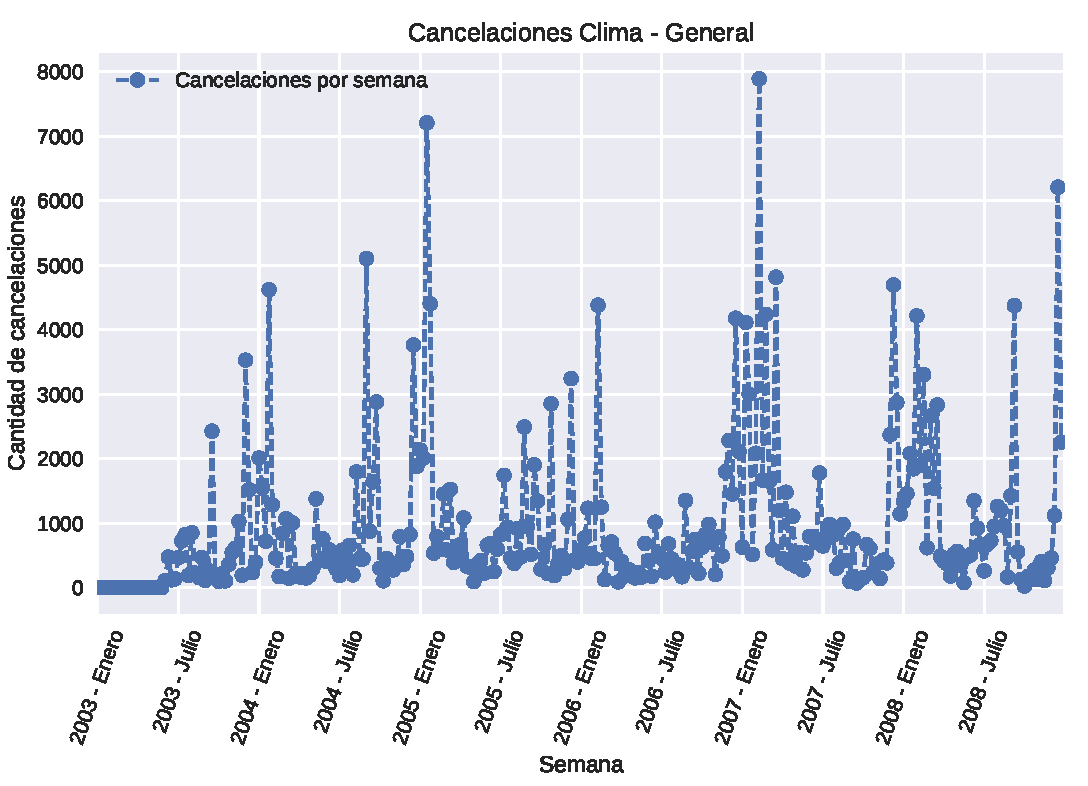
\includegraphics[scale=0.62]{diapos/imagenes/cancelacionesClimaGeneralPlotV1.pdf}
}

\end{frame}

% -----------------------------------


\begin{frame}

% Por que senos y cosenos, hablar de la periodicidad
% Vemos que un periodo se repite cada año (48 semanas)
% Queremos tener en cuenta periodos semestrales
% La familia que utilizamos fue esta porque bla (lo explicado antes)
% Contar lo de la elevacion a la potencia

% No hay mucho mas que decir

\frametitle{Familia de funciones}

\pause

% \begin{align}
$$f(t) = \alpha_1 + \alpha_2 * cos(\frac{2\pi}{48} t)^{8} + \alpha_3 * sen(\frac{2\pi}{24} t) + \alpha_4 * sen(\frac{2\pi}{12} t)$$
% \end{align}

\end{frame}

% -----------------------------------


\begin{frame}

\frametitle{Resultados - General}

% Las cosas no fueron exactas blabla contar el grafico

{\centering
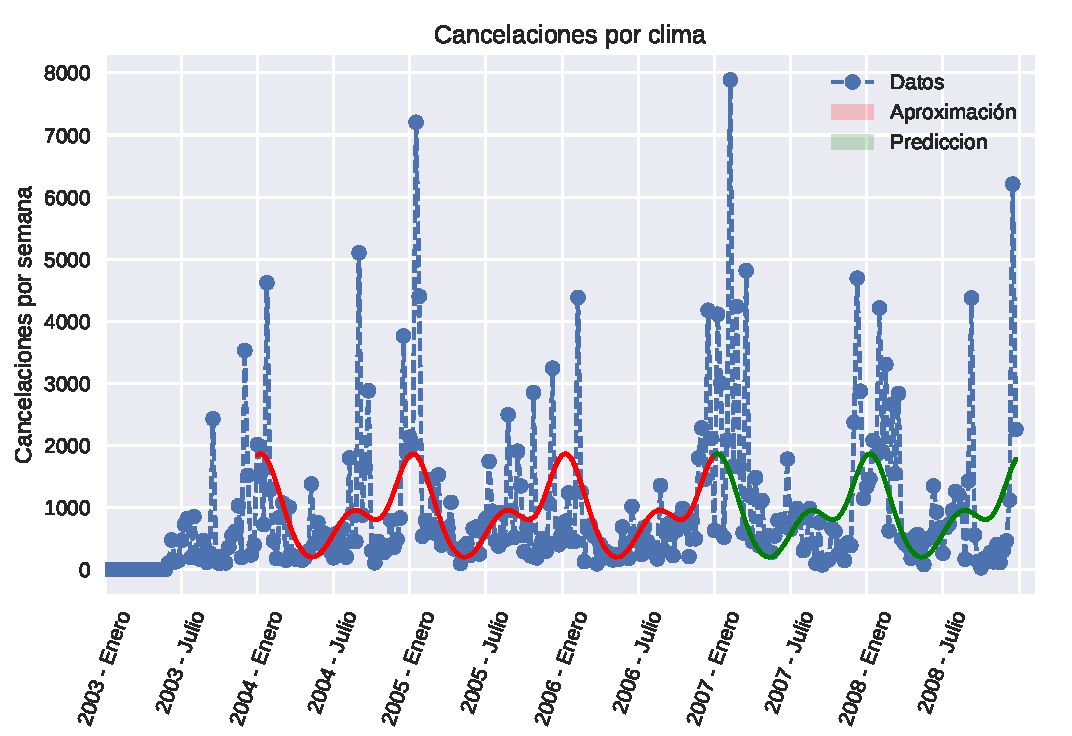
\includegraphics[scale=0.62]{diapos/imagenes/cancelacionesPorClimaGeneralPrediccionV1.pdf}
}


\end{frame}

% -----------------------------------

\begin{frame}

\frametitle{Resultados - Miami outliers}

% Como lo anterior podia tener mucho "ruido" de muchos aeropuertos, nos especializamos en dos.
% Ver informe por razones de eleccion, etc

% Francisco me tiro la idea que podemos mostrar miami con/sin outliers para mostrar la diferencia

\todo[inline]{Quiza no valga la pena mostrar lo de los outliers}
{\centering
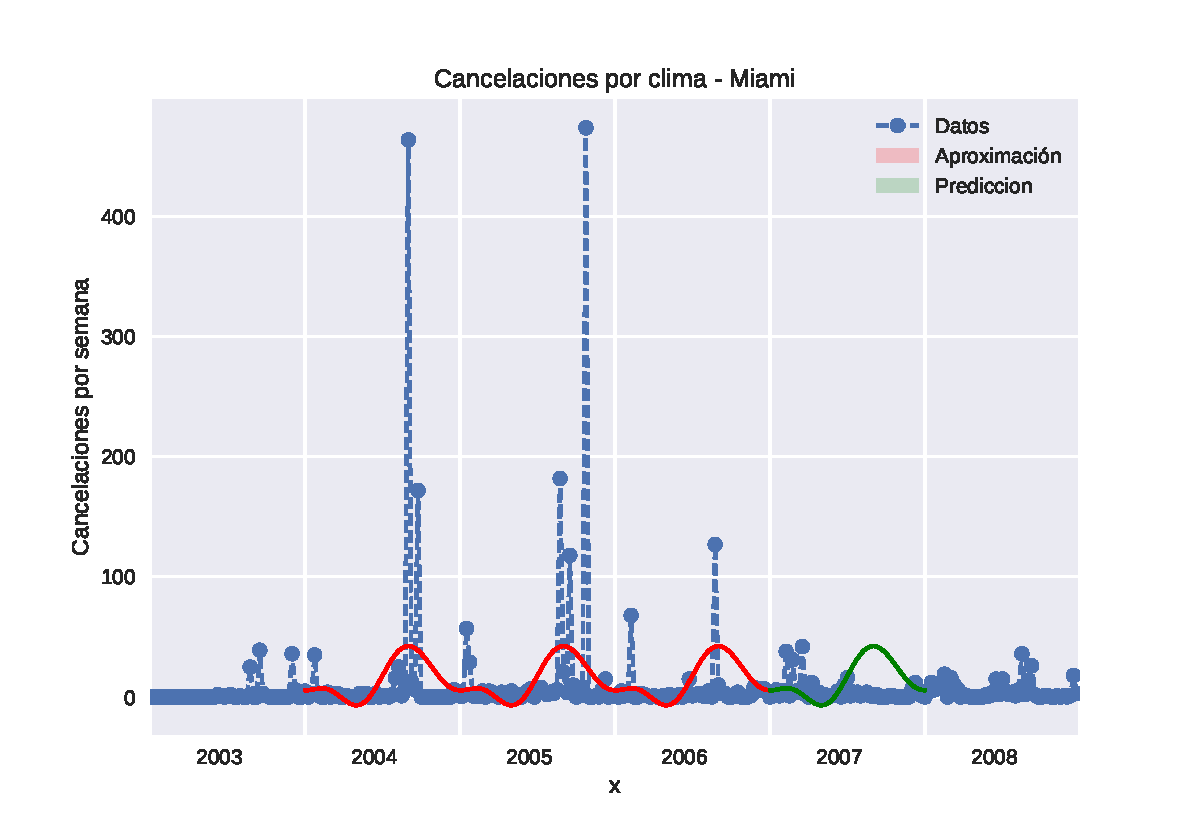
\includegraphics[scale=0.62]{diapos/imagenes/cancelacionesClimaMiamiPrediccionCONOUTS.pdf}
}

\end{frame}

% -----------------------------------

\begin{frame}

\frametitle{Resultados - Miami y Los Ángeles}

% Como lo anterior podia tener mucho "ruido" de muchos aeropuertos, nos especializamos en dos.
% Ver informe por razones de eleccion, etc

% IMPORTANTE: CONCLUIR ALGO
{\centering
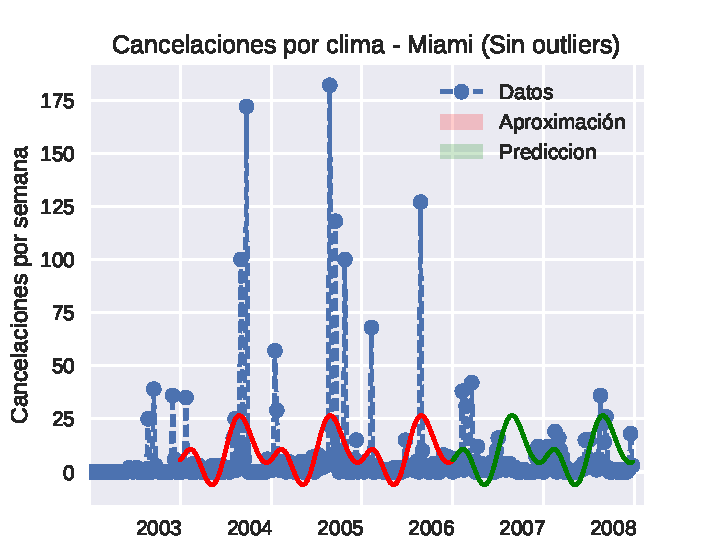
\includegraphics[scale=0.5]{diapos/imagenes/cancelacionesClimaMiamiPrediccionV1SINOUTS.pdf}
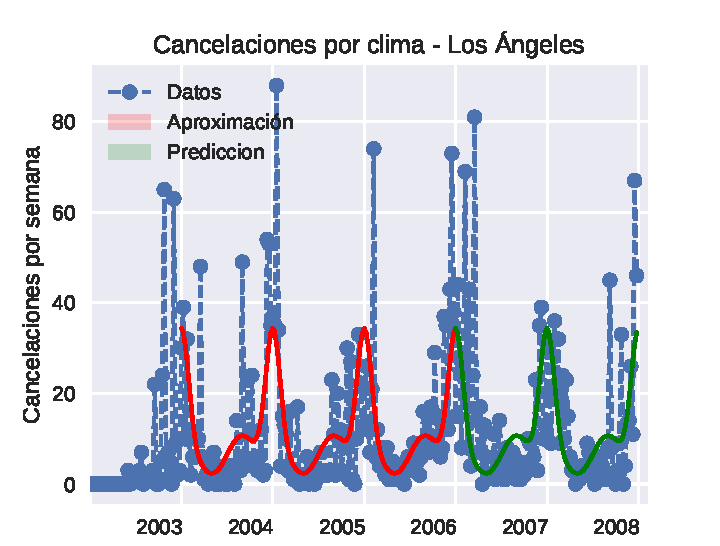
\includegraphics[scale=0.5]{diapos/imagenes/cancelacionesClimaLosAngelesPrediccionV1.pdf}
}

\end{frame}

% -----------------------------------

\begin{frame}

\frametitle{Conclusiones}

\begin{itemize}
\item{Picos en diciembre y enero. Tormentas de Agosto.}
\item{Diferencias entre aeropuertos.}
\item{Exacticud del método.}
\end{itemize}

\end{frame}

% -----------------------------------

\begin{frame}

% Explicar el eje, ver informe, no hay mucho mas
% Desarrollar un poco ante cada pregunta

\frametitle{Aerolíneas}

\begin{itemize}
    \item{¿Cómo se comporta nuestro modelo con la cantidad de retrasos por aerolíneas?}
    \item{¿Es posible predecir alguna mejor que otra?}
    \item{¿Será necesario adaptar la familia de funciones cada vez?}
\end{itemize}

\end{frame}

% -----------------------------------

\begin{frame}

% Fijamos aeropuertos por la gran variacion, elegimos los mas grandes por razones
% Consideramos que un retraso es tal cosa
% Basicamente el preliminar del informe, ver eso

\frametitle{Aerolíneas - Intro}

\begin{itemize}
    \item{Aeropuertos fijos.}
    \item{Elección de aeropuertos y aerolíneas.}
    \item{Clasificación de retrasos.}
\end{itemize}

\end{frame}


% -----------------------------------

\begin{frame}

% Explicar la familia de funciones, simil informe

\frametitle{United Airlines - Funciones}

$$ f(t) = \alpha_1 + \alpha_2 * t + \alpha_3 * cos(\frac{2\pi}{48} t) + \alpha_4 * cos(\frac{2\pi}{24} t) + \alpha_5 * cos(\frac{2\pi}{12} t) $$

\end{frame}


% -----------------------------------

\begin{frame}

% Explicar los graficos


\frametitle{United Airlines - Los Ángeles}

{\centering
  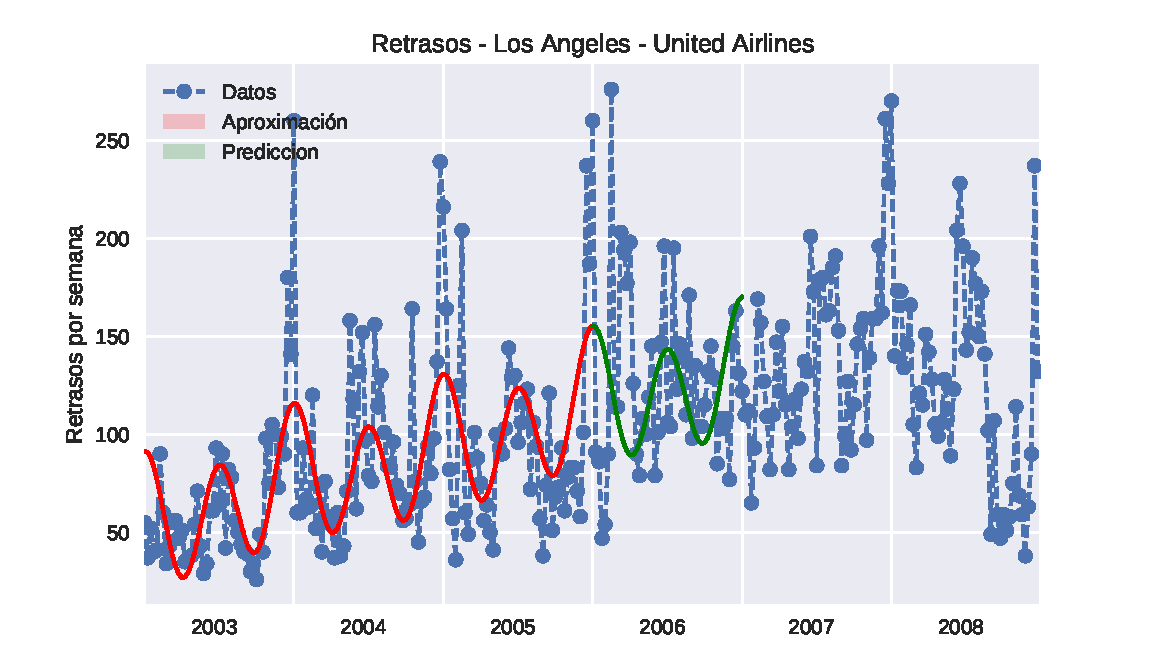
\includegraphics[width=1.0\linewidth]{diapos/imagenes/retrasosUnitedAirlinesLAvol3.pdf}
}

\end{frame}

% -----------------------------------

\begin{frame}

% Explicar los graficos

\frametitle{United Airlines - Atlanta}

{\centering
  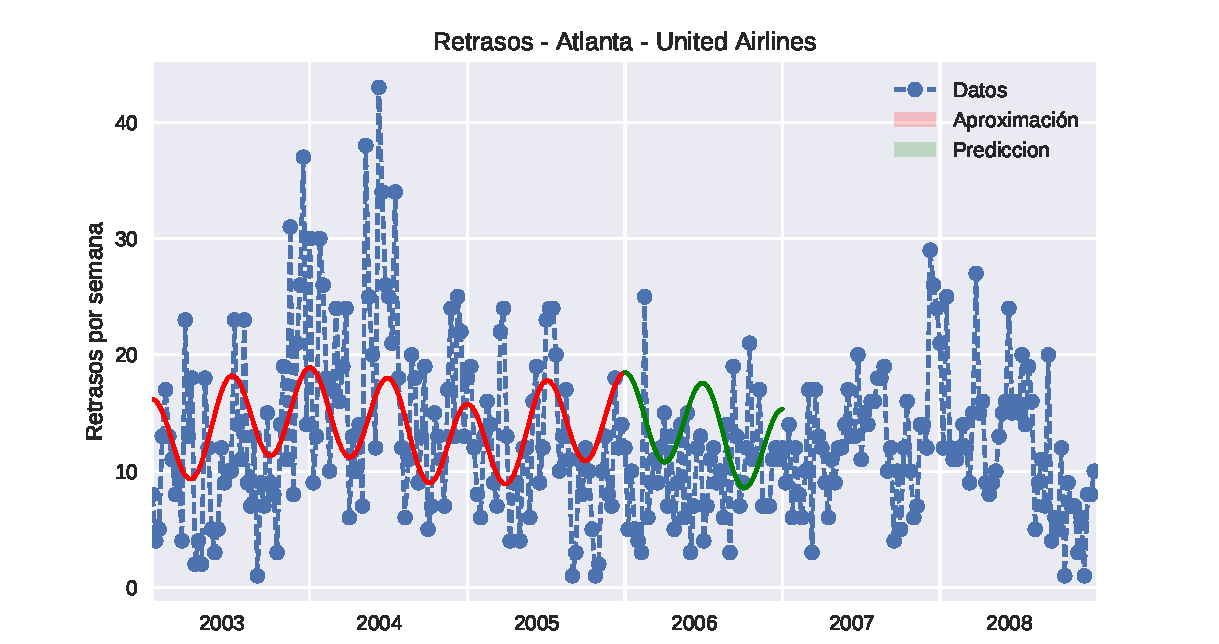
\includegraphics[width=1.0\linewidth]{diapos/imagenes/retrasosUnitedAirlinesATLvol3.pdf}
}

\end{frame}

% -----------------------------------

\begin{frame}

% Conclusiones sobre los graficos anteriores
% IMPORTANTE: La misma funcion minimiza distintos aeropuertos, patrones se repiten
% ver informe

\frametitle{United Airlines - Analisis}

\begin{itemize}

\item{Funciones periódicas consiguieron el mínimo.}
\item{Misma familia minimizó varios aeropuertos.}
\item{Queremos ver si este comportamiento se repite en otra aerolínea.}

\end{itemize}

\end{frame}

% -----------------------------------

\begin{frame}

% Explicar los graficos
% Conclusiones sobre ellos
% IMPORTANTE: La misma funcion minimiza distintos aeropuertos, patrones se repiten
% ver informe

\frametitle{American Airlines - Los Ángeles}

{\centering
  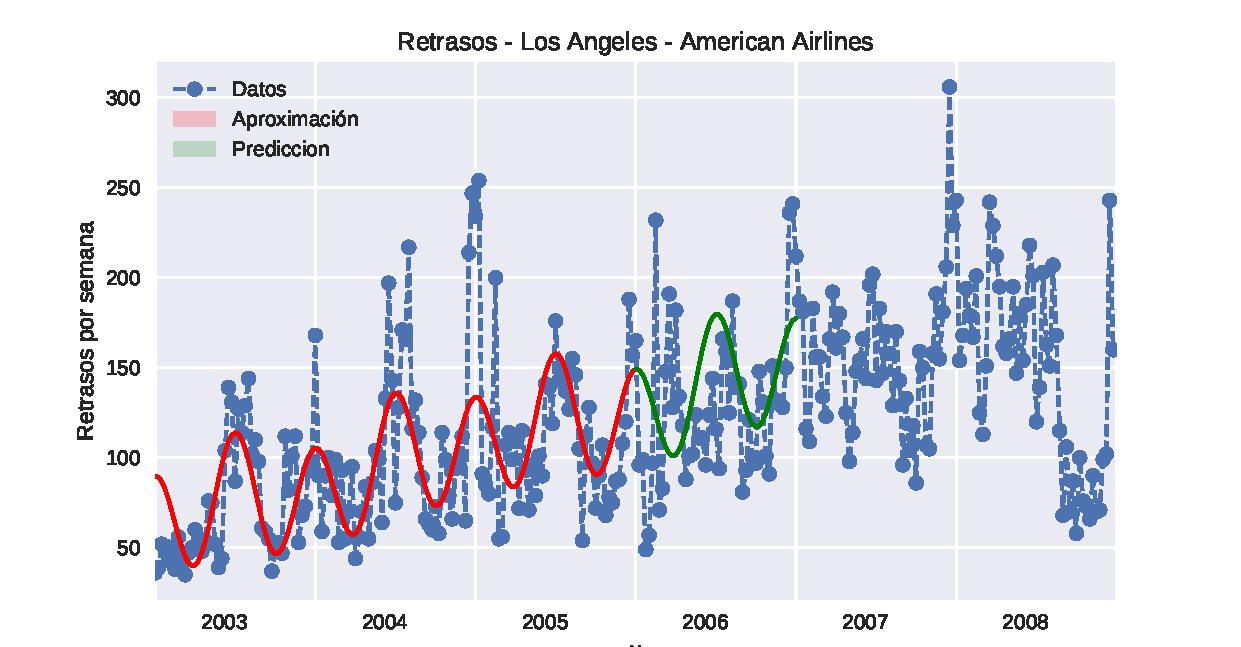
\includegraphics[width=1.0\linewidth]{diapos/imagenes/retrasosAmericanAirlinesLAvol3.pdf}
}

\end{frame}

% -----------------------------------

\begin{frame}

% Explicar los graficos
% Conclusiones sobre ellos
% IMPORTANTE: La misma funcion minimiza distintos aeropuertos, patrones se repiten
% ver informe

\frametitle{American Airlines - Atlanta}

{\centering
  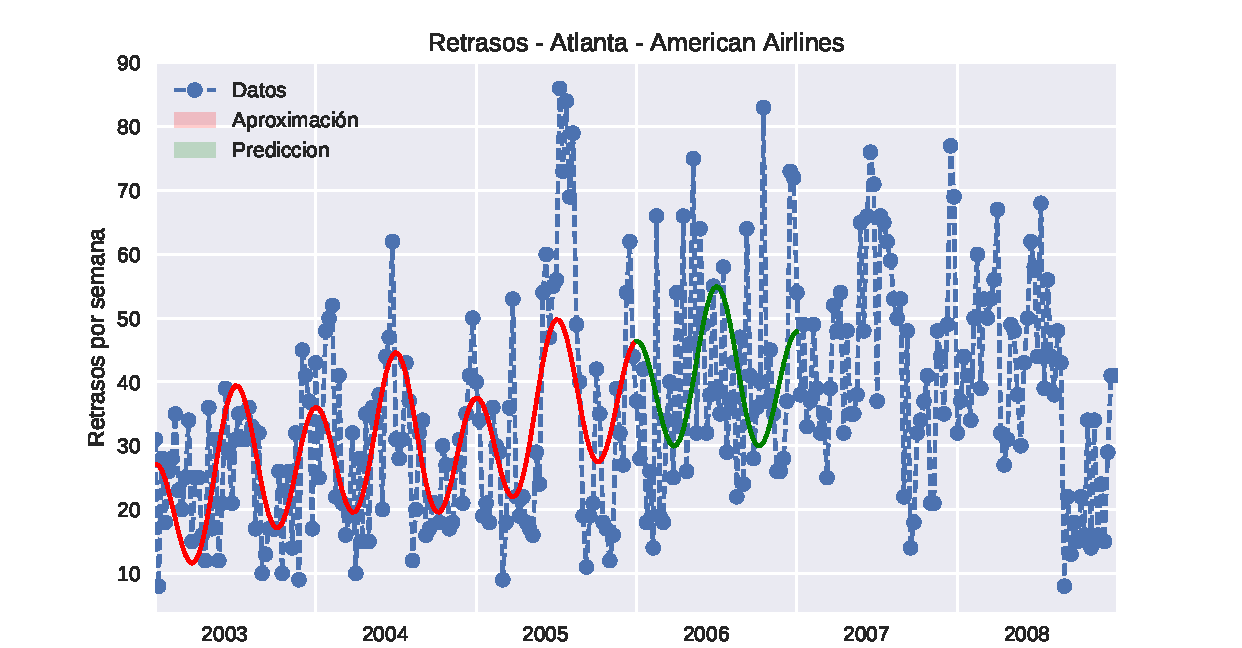
\includegraphics[width=1.0\linewidth]{diapos/imagenes/retrasosAmericanAirlinesATLvol3.pdf}
}

\end{frame}

% -----------------------------------

\begin{frame}

\frametitle{Conclusiones}

% Conclusiones finales sobre el eje, ver informe

\begin{itemize}
    \item{Periodicidad.}
    \item{Patrones generales.}
    \item{Uso de la misma familia de funciones.}
\end{itemize}


\end{frame}



% \begin{frame}
% \frametitle{Ejemplo del comando \textbackslash item}

% \begin{itemize}
%     \item<1-> {Para llegar a la solución tenemos que probar diferentes posibilidades.}
%     \item<2-> {Una forma de encarar el problema es pensar en las decisiones que pude haber tomado para llegar a mi posición actual.}
%     \item<3-> {En nuestro caso, si estoy parado en una cierta casilla \textbf{solamente} pude haber llegado desde la casilla de \textbf{arriba} o desde la \textbf{izquierda}.}
%     \item<4> {\textit{Cuidado con los bordes}. Por ejemplo, si estamos en el borde izquierdo solo pudimos venir desde arriba. Ignoremos los casos borde por unos momentos}

% \end{itemize}

% \end{frame}

% % ------------------------------

% \begin{frame}
% \frametitle{Ejemplo del comando pause}

% % Con la observación en mente, ya sabemos como se relacionan las casillas en un camino mínimo. \\
% % \pause
% Queremos encontrar el peso del camino mínimo que va desde (1,1) hasta (m,n). Pongámosle nombre a lo que buscamos.\\
% \pause
% \begin{block}{Definición}
% f(i, j) = Peso del camino mínimo que va desde (1,1) hasta (i,j).
% \end{block}
% \pause
% $ $\newline
% La solución a nuestro problema es f(m, n).
% \end{frame}





%------------------------------------------------

\begin{frame}
\Huge{\centerline{Preguntas}}
\end{frame}

%----------------------------------------------------------------------------------------

\end{document}